\documentclass[pdf, aspectratio=169, 12pt]{beamer}
\usepackage[]{hyperref, graphicx, siunitx, lmodern, tikz, booktabs, physics, multicol}
\usepackage[mode=buildnew]{standalone}
\usepackage{pdfpc-commands}
\usepackage{pgfplots}
\pgfplotsset{compat=1.16}

\usetheme{Python}

\graphicspath{ {Images/} }

\sisetup{per-mode=symbol}
\usetikzlibrary{calc, patterns, decorations.markings, decorations.pathmorphing, shapes}

%Preamble
\title{It's Hereditary}
\author{Jed Rembold}
\date{April 1, 2020}

\begin{document}

\begin{frame}{Announcements}
	\begin{itemize}
		\item Homework
			\begin{itemize}
				\item Remember that HW8 was postponed to be due next week!
			\end{itemize}
		\item Be working on your Midterm projects/scripts
			\begin{itemize}
				\item Due Friday night at midnight
			\end{itemize}
		\item I'm trying desperately to get caught up on grading, but it has been an uphill battle
		\item I'm aiming to get updated grade reports pushed to WISE as soon as I can, but if you need to know where you are at before Friday so you can make an educated decision about C/NC, just let me know and I'll make you a priority.
		\item Polling: \nolinkurl{rembold-class.ddns.net}
	\end{itemize}
\end{frame}

\begin{frame}[fragile]{Review Question}
	\begin{columns}
		\column{0.4\textwidth}
		Suppose you run the bit of code to the right. What would the printed output be?
		\vspace{5mm}
		\begin{poll}
		\item \pyi[output]{Spot is 8!}
		\item \pyi[output]{Dog(Spot,8)}
		\item \pyi[output]{Waffles is 6!}
		\item This code would give an error.
		\end{poll}
		\exsol{\pyi[output]{Spot is 8!}}

		\column{0.68\textwidth}
		\footnotesize
		\begin{pythoncode}
			class Dog:
				def __init__(self, name, age):
					self.name = name
					self.age = age
				def __repr__(self):
					return f'Dog({self.name},{self.age})'
				def __str__(self):
					return f'{self.name} is {self.age}!'

			A = Dog('Waffles', 6)
			B = Dog('Spot', 8)
			if str(A) == str(B):
				print(A)
			else:
				print(B)
		\end{pythoncode}
	\end{columns}
\end{frame}

\begin{frame}{Defining vs Using}
	\begin{columns}[t]
		\column{0.5\textwidth}
		\begin{block}{Defining the Class}
			\begin{itemize}
				\item \alert{Implement} a new object type with a class
					\begin{itemize}
						\item define the class
						\item define \alert{data attributes}
							\begin{itemize}
								\item \textcolor{Red}{What is} the object?
							\end{itemize}
						\item Define \alert{methods}
							\begin{itemize}
								\item \textcolor{Red}{How to} use the object?
							\end{itemize}
					\end{itemize}
			\end{itemize}
		\end{block}
		\column{0.5\textwidth}
		\begin{block}{Using the Class}
			\begin{itemize}
				\item \alert{Using} the new object type in the code
					\begin{itemize}
						\item Create \alert{instances} of the object type
						\item Do \alert{operations} with them
					\end{itemize}
			\end{itemize}
		\end{block}
		
	\end{columns}
\end{frame}

\begin{frame}{Type vs Instance}
	\begin{columns}[t]
		\column{0.5\textwidth}
		\begin{block}{The Type}
			\begin{itemize}
				\item Class name is the \alert{type}
				\item Class is defined generically
					\begin{itemize}
						\item Use \pyi{self} to refer to some instance 
						\item \pyi{self} is a parameter to our methods 
					\end{itemize}
				\item The class defines data and method common across \alert{all} instances
			\end{itemize}
		\end{block}
		\column{0.5\textwidth}
		\begin{block}{The Instance}
			\begin{itemize}
				\item Instance in one \alert{specific} object
				\item Data attributes vary between instances
				\item Instance has the same structure as the class
			\end{itemize}
		\end{block}
	\end{columns}
\end{frame}

\begin{frame}{Internal Representation}
	\begin{itemize}
		\item Fundamental idea of types was \alert{internal} representation
		\item We interact with the object through methods, the class takes care of manipulating the internal representation.
		\item Python is not great at enforcing this:
			\begin{itemize}[<+->]
				\item We can \alert{access} data attributes from outside the class definition
					\begin{itemize}
						\item \pyi{print(a1.age)}
					\end{itemize}
				\item We can \alert{alter} data attributes from outside the class definition
					\begin{itemize}
						\item \pyi{a1.age = 5000}
					\end{itemize}
				\item We can \alert{create new} data attributes from outside the class definition
					\begin{itemize}
						\item \pyi{a1.is_awesome = True}
					\end{itemize}
			\end{itemize}
	\end{itemize}
\end{frame}

\begin{frame}{Just because you CAN\ldots}
	\begin{itemize}
		\item In practice, it is generally a poor idea to do any of these things
		\item A programmer may need to change the internal representation to implement a new feature or fix a bug
			\begin{itemize}
				\item If your program directly accessed that representation, it is probably now broken.
			\end{itemize}
		\item Methods are our way of interacting with an object, so if you want to get or set a data attribute, write a method for it!
			\begin{itemize}
				\item Commonly called getters and setters
			\end{itemize}
	\end{itemize}
\end{frame}

\begin{frame}{Private and Protected}
	\begin{itemize}
		\item It \emph{is} possible to declare certain data attributes to be either private or protected
			\begin{itemize}
				\item Really more a warning or recommendation that enforcement
				\item Still possible to access and change those attributes, just a bit harder
				\item Nothing is truly private in Python
			\end{itemize}
		\item<2-> Private data attribute names prefixed with 2 underscores
			\begin{itemize}
				\item \pyi{self.__myval = 5}
				\item Only accessible (easily) within that specific class
			\end{itemize}
		\item<3-> Protected data attribute names prefixed with a single underscore
			\begin{itemize}
				\item \pyi{self._myval = 5}
				\item Accessible within that class and future sub-classes
			\end{itemize}
	\end{itemize}
\end{frame}

\begin{frame}{More a set of guidelines really\ldots}
	\begin{itemize}
		\item Setting attributes to be private or protected isn't a guarantee that they can't be viewed, accessed, or modified!
		\item Think of it more as a reminder to future you (or other coders) if certain values should be allowed to be accessed outside the class definition.
	\end{itemize}
\end{frame}

\begin{frame}{Inheritance}
	\begin{itemize}
		\item Classes are already about grouping similar types of objects together
		\item Groups of objects are frequently related to other groups of objects
			\begin{itemize}
				\item Either as a subset or a superset
			\end{itemize}
		\item We can mimic and take advantage of these relationships in our classes!
	\end{itemize}
\end{frame}

\begin{frame}{Hierarchy Example}
	\vspace{5mm}
	\begin{center}
		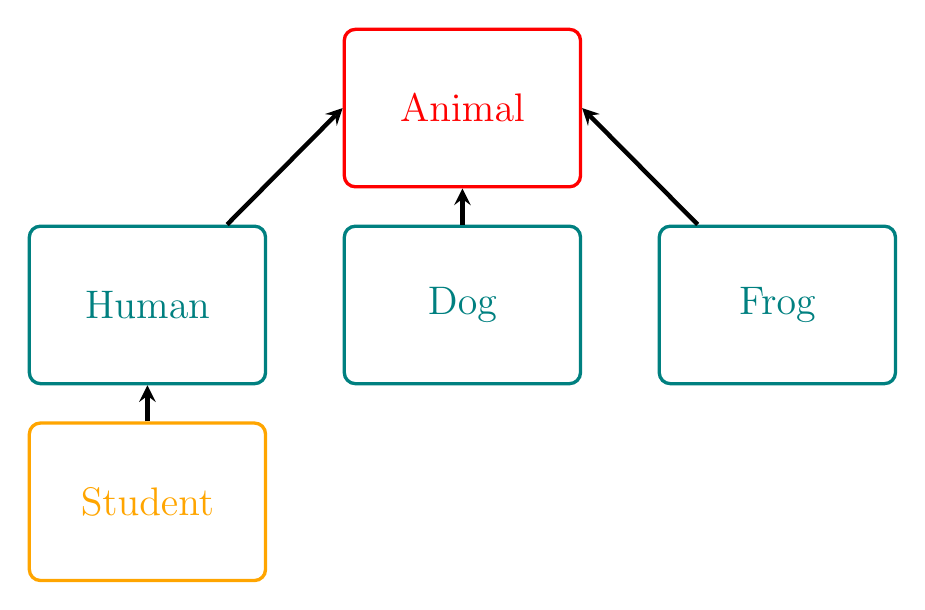
\begin{tikzpicture}[
			every node/.style={minimum width=3cm, minimum height=2cm, rounded corners, draw, very thick, font=\Large},
			]
			\node[Red](an) at (0,0) {Animal};

			\node[Teal](hum) at (-4,-2.5) {Human};
			\node[Teal](dog) at (0,-2.5) {Dog};
			\node[Teal](frog) at (4,-2.5) {Frog};
			\path[-stealth, ultra thick] (hum) edge (an.west)
							(dog) edge (an.south)
							(frog) edge (an.east);

			\node[Orange](stud) at (-4,-5) {Student};
			\draw[-stealth, ultra thick] (stud) -- (hum.south);
		\end{tikzpicture}
	\end{center}
\end{frame}

\begin{frame}{Hierarchy Terms}
	\begin{itemize}
		\item Arrows point toward the \alert{parent class} or superclass
		\item Arrows point from a \alert{child class} or subclass
			\begin{itemize}
				\item \alert{Inherit} all data attributes and methods from parent class
				\item Can have new attributes added
				\item Can have new methods added
				\item Can have parents methods overridden
			\end{itemize}
		\item Children specify who their parents are (not vice versa)
	\end{itemize}
\end{frame}

\begin{frame}{Name your parent (in code)}
	\begin{itemize}
		\item We specify what a class's parent is immediately following the class's name
			\begin{itemize}
				\item Surround parent's name is parentheses
				\item \pyi{class Human(Animal):}
				\item The default parent is type \pyi{object}
			\end{itemize}
	\end{itemize}
\end{frame}
\end{document}

